% !TeX spellcheck = en_US
\addsection{Random Scenario}{\images/random.png}

\begin{multicols}{2}

\textit{As dice roll and fortunes shift, the lands of Antagarich spread before you in all their splendor.
  Your destiny follows these celestial rolls, each battle and treasure determined by chance.
  Will you emerge victorious in this battle royale, claim the sacred grail, or stand alone as the king of the hill when the final die settles?  % no-check-caps
}

Instead of playing a specific Scenario, you can follow these guidelines to create a random one.
Of course, you can adjust everything at will.

\subsection*{\MakeUppercase{Scenario Type}}

Choose one of the following types for your play:

\textbf{Free-for-All} -- Win by eliminating your opponents or gaining more Victory Points (VPs) than them.
VPs are counted in accordance to the Tournament book.
Additionally, you get:
\begin{itemize}
  \item 5 VPs for flagging a Dragon Utopia for the first time.
  \item 2 VPs for controlling the Dragon Utopia at the end of the game.
  \item 5 VPs for bringing the Grail to your Faction Town \textit{OR} 3 VPs for owning the Grail  at the end of the game.
\end{itemize}

\textbf{King of the Hill} -- Start a map with a Dragon Utopia in the middle.
You don't need to fight the Level 7 Combat to capture it.
You get 1 VP for each Round you hold the Dragon Utopia under your control, no VPs from anything else.

\textbf{Capture the Grail} -- Start a map with the Grail in the middle.
Standard Grail rules apply: spend 2 \svgeven{movement} to dig it up, and bring it to your Town.
\vspace*{\fill}
\columnbreak

\subsection*{\MakeUppercase{Map Size}}

\textbf{Small (S) Map:} 8 Rounds, and give every player:
\begin{itemize}
  \item 1 × Starting (I) Map Tile
  \item 2 × Far (II-III) Map Tile
\end{itemize}

\textbf{Medium (M) Map:} 12 Rounds, and give every player:
\begin{itemize}
  \item 1 × Starting (I) Map Tile
  \item 2 × Far (II-III) Map Tile
  \item 1 × Near (IV-V) Map Tile
\end{itemize}

\textbf{Large (XL) Map:} 16 Rounds, and give every player:
\begin{itemize}
  \item 1 × Starting (I) Map Tile
  \item 2 × Far (II-III) Map Tile
  \item 2 × Near (IV-V) Map Tile
\end{itemize}

\medskip

\hommtablemulticol[]{19}{
  \centering
  \medskip
  \textbf{Central Map Tile(s)}\\
  \bigskip
  \hspace{-0.7em}
  \begin{tabularx}{0.99\linewidth}{p{1.7em}>{\centering\arraybackslash}X>{\centering\arraybackslash}X>{\centering\arraybackslash}X} & \darkcell[1.4]{Free-for-All} & \darkcell[1.4]{King of the Hill} & \darkcell[1.4]{Capture the Grail} \\
    \darkcell[1.8]{S}
    & \lightcell[1.8]{
\includegraphics[width=0.75\linewidth]{\maps/near-tile.png}}
    & \multirow{3}{*}[7.6ex]{\parbox{\linewidth}{\centering\lightcell[6.19]{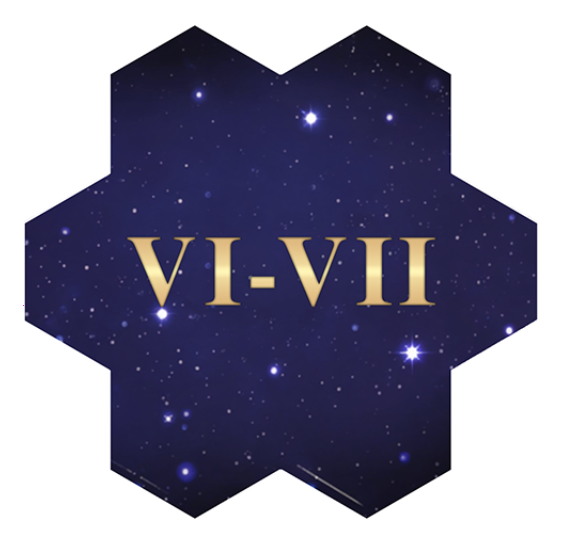
\includegraphics[width=0.75\linewidth]{\maps/center-tile.png} with a Dragon Utopia (C1 or C3)}}}
    & \multirow{3}{*}[7.6ex]{\parbox{\linewidth}{\centering\lightcell[6.19]{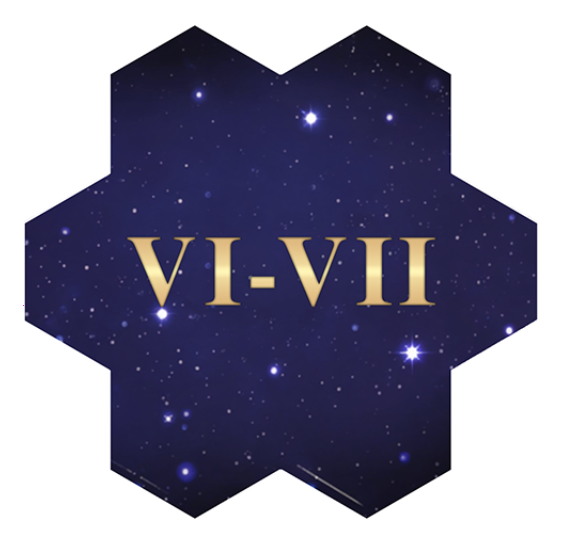
\includegraphics[width=0.75\linewidth]{\maps/center-tile.png} with a\linebreak Grail\linebreak (C2 or C4)}}} \\
    \darkcell[2.2]{M}
    & \lightcell[2.2]{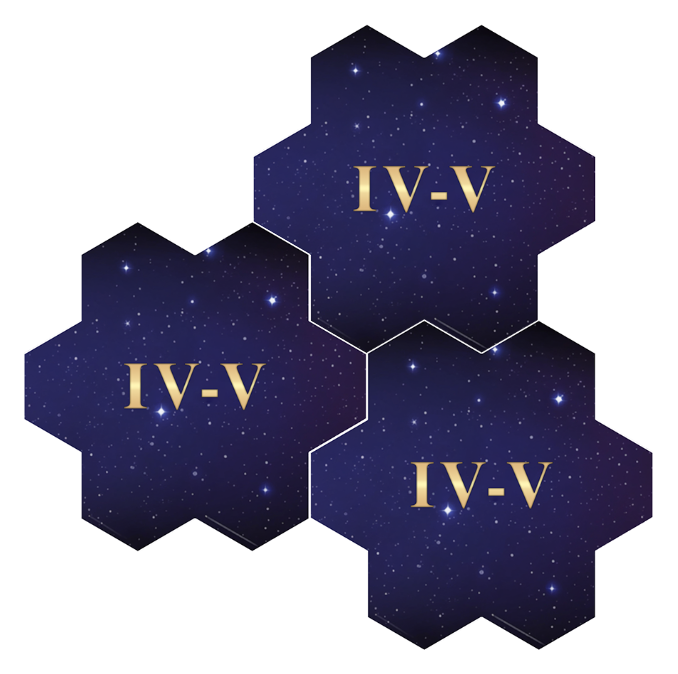
\includegraphics[width=0.95\linewidth]{\maps/medium.png}}
    &
    & \\
    \darkcell[1.8]{XL}
    & \lightcell[1.8]{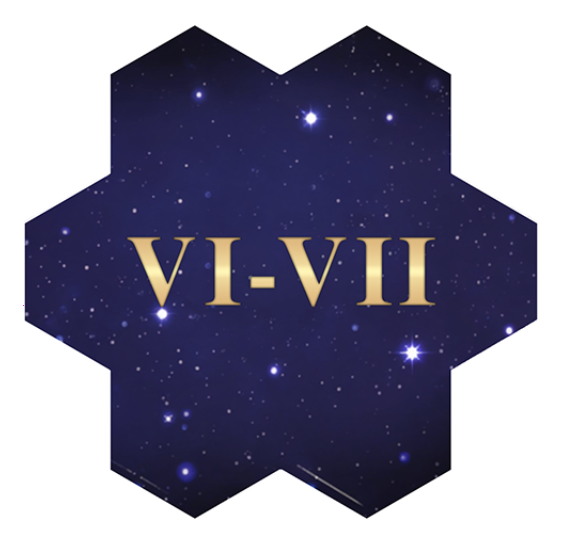
\includegraphics[width=0.75\linewidth]{\maps/center-tile.png}}
    &
    & \\
  \end{tabularx}
}

\end{multicols}

\vspace{-3\baselineskip}

\subsection*{\MakeUppercase{Map Setup}}

\definecolor{castlebg}{RGB}{25,85,196}
\definecolor{infernobg}{RGB}{190,21,38}
\definecolor{rampartbg}{RGB}{53,192,56}

First, place the Central Map Tile(s) for your Scenario type and size in the middle.
Decide player order before placing the remaining Tiles.
In reverse player order, each player places one Tile in descending level (Near \rightarrow\ Far \rightarrow\ Starting).  % no-check-caps
Every new Tile needs to connect to at least one existing Tile.

The following \textbf{example} shows building the map for a \textbf{3-player XL Free-for-All}, with player 1 playing as \textcolor{rampartbg}{\textbf{Rampart}}, player 2 as \textcolor{infernobg}{\textbf{Inferno}}, and player 3 as \textcolor{castlebg}{\textbf{Castle}}.
First, put the Center (VI-VII) Map Tile in the middle, and then proceed to distribute Near (IV-V) Map Tiles in the following order:

\bigskip

% Create a command for player images with horizontal padding
\newcommand{\playerimage}[2]{%
  \begin{minipage}[t]{0.28\textwidth} % Slightly narrower to create padding
    \centering
    \includegraphics[width=0.9\linewidth]{#1} % Images at 90% of column width for padding
    \captionof{figure}{\large\textbf{#2}}
  \end{minipage}%
}

\newcommand{\playerarrow}[4]{%
  % #1 = x-offset from current position
  % #2 = y-offset from current position
  % #3 = rotation angle in degrees
  % #4 = arrow color
  \tikz[remember picture, overlay, baseline=(current bounding box.base)] {
    \coordinate (here) at (0,0);
    \draw[-Triangle, ultra thick, #4, opacity=0.8]
      ([shift={(#1,#2)}]here) -- ++({#3}:0.8cm);
  }%
}

% Save the content in a box to measure its dimensions
\newsavebox{\contentbox}
\begin{lrbox}{\contentbox}
\begin{minipage}{\textwidth}
  % Header
  \noindent
  \rule{\textwidth}{0pt}
  \hspace{0.01\textwidth} % Add left margin
  \rule{\textwidth}{0pt}
  \begin{minipage}{\textwidth/3}
    \centering
    \textbf{\textcolor{castlebg}{Player 3: Castle}}
  \end{minipage}%
  \hfill
  \begin{minipage}{\textwidth/3}
    \centering
    \hspace{1em}\textbf{\textcolor{infernobg}{Player 2: Inferno}}
  \end{minipage}%
  \hfill
  \begin{minipage}{\textwidth/3}
    \centering
    \hspace{1.5em}\textbf{\textcolor{rampartbg}{Player 1: Rampart}}
  \end{minipage}%
  \vspace{1em}
  % First row
  \noindent
  \hspace{0.01\textwidth} % Add left margin
  \playerimage{\maps/free-for-all-xl-1.png}{1}%
  \playerarrow{-2.8}{0.2}{60}{castlebg}
  \hfill
  \playerimage{\maps/free-for-all-xl-2.png}{2}%
  \playerarrow{-1.5}{0.2}{160}{infernobg}
  \hfill
  \playerimage{\maps/free-for-all-xl-3.png}{3}
  \playerarrow{-4.3}{2.6}{-60}{rampartbg}
  \hspace{0.01\textwidth} % Add right margin
  \begin{center}
    \color{darkgray}{\rule{0.98\textwidth}{0.5pt}}
  \end{center}
  \vspace{1em}

  % Second row
  \noindent
  \hspace{0.01\textwidth} % Add left margin
  \playerimage{\maps/free-for-all-xl-4.png}{4}%
  \playerarrow{-3.2}{3.2}{-30}{castlebg}
  \hfill
  \playerimage{\maps/free-for-all-xl-5.png}{5}%
  \playerarrow{-0.8}{1.4}{210}{infernobg}
  \hfill
  \playerimage{\maps/free-for-all-xl-6.png}{6}
  \playerarrow{-3.6}{1.2}{120}{rampartbg}
  \hspace{0.01\textwidth} % Add right margin
  \begin{center}
    \color{darkgray}{\rule{0.98\textwidth}{0.5pt}}
  \end{center}
\end{minipage}
\end{lrbox}

% Draw the background columns based on content dimensions
\begin{tikzpicture}
  % Calculate content height
  \newlength{\contentheight}
  \setlength{\contentheight}{\ht\contentbox}
  \addtolength{\contentheight}{\dp\contentbox}

  % Draw the background columns with fixed positions and extra padding
  % Moving columns slightly to align better with the padded content
  \fill[castlebg, opacity=0.1] (0.01\textwidth,0) rectangle (0.31\textwidth,-\contentheight);
  \fill[infernobg, opacity=0.1] (0.36\textwidth,0) rectangle (0.66\textwidth,-\contentheight);
  \fill[rampartbg, opacity=0.1] (0.71\textwidth,0) rectangle (0.99\textwidth,-\contentheight);

  % Place the content
  \node[inner sep=0pt, anchor=north west] at (0,0) {\usebox{\contentbox}};
\end{tikzpicture}

\vspace{1em}

Then, keeping the same order, place Far (II-III) Map Tiles, and finally Starting (I) Map Tiles:

\vspace{1em}

\begin{minipage}{\textwidth}
  \noindent
  \hspace{0.01\textwidth} % Add left margin
  \playerimage{\maps/free-for-all-xl-far-1.png}{7}%
  \playerarrow{-4.4}{3.8}{-30}{rampartbg}
  \playerarrow{-3.9}{-0.3}{60}{infernobg}
  \playerarrow{-0.6}{4.0}{-120}{castlebg}
  \hfill
  \playerimage{\maps/free-for-all-xl-far-2.png}{8}%
  \playerarrow{-4.7}{4.3}{-60}{rampartbg}
  \playerarrow{-5.2}{-0.1}{30}{infernobg}
  \playerarrow{-0.9}{4.3}{-150}{castlebg}
  \hfill
  \playerimage{\maps/free-for-all-xl-finish.png}{9}
  \playerarrow{-5.2}{4.3}{-30}{rampartbg}
  \playerarrow{-5.5}{0.9}{30}{infernobg}
  \playerarrow{-0.3}{4.3}{-150}{castlebg}
  \hspace{0.01\textwidth} % Add right margin
\end{minipage}

\begin{center}
  \color{darkgray}{\rule{0.98\textwidth}{0.5pt}}
\end{center}

\pagebreak


\subsection*{\MakeUppercase{Player Setup}}

Choose your \textbf{starting conditions} and \textbf{Town strength}.

\let\origbronze\bronze
\let\origsilver\silver
\let\origgolden\golden
\let\origazure\azure
\renewcommand{\bronze}{\origbronze[12]}
\renewcommand{\silver}{\origsilver[12]}
\renewcommand{\golden}{\origgolden[12]}
\renewcommand{\azure}{\origazure[12]}


\hommtable[]{27}{
  \centering
  \medskip
  \textbf{Starting Conditions}\\
  \bigskip

  \begin{tabularx}{0.99\linewidth}{p{0.12\linewidth}XXXX} & \darkcell{Stingy} & \darkcell{Fair} & \darkcell{Generous}\\
  \darkcell[1.4]{Army}
    & \lightcellleft[1.4]{2 × Few cheapest \bronze\ Units}
    & \lightcellleft[1.4]{Pack of cheap \bronze\ Units \linebreak Few chosen \bronze\ Units}
    & \lightcellleft[1.4]{Pack of chosen \bronze\ Units \linebreak Few cheap \silver\ Units}\\
  \darkcell[1.4]{Starting Resources}
    & \lightcellleft[1.4]{10 \svg{gold}, 3 \svg{building_materials}, 1 \svg{valuables}}
    & \lightcellleft[1.4]{16 \svg{gold}, 5 \svg{building_materials}, 1 \svg{valuables}}
    & \lightcellleft[1.4]{20 \svg{gold}, 8 \svg{building_materials}, 2 \svg{valuables}}\\
  \end{tabularx}

  \bigskip
  {\color{\iftoggle{noartbackground}{black}{darkyellow}}\rule{\textwidth}{0.5pt}}

  \vspace*{1em}
  \textbf{Town Strength}\\
  \bigskip

  \begin{tabularx}{0.99\linewidth}{p{0.12\linewidth}XXXX} & \darkcell{Settlement} & \darkcell{City} & \darkcell{Capitol}\\
  \darkcell[1.4]{Starting Income}
    & \lightcellleft[1.4]{10 \svg{gold}, 0 \svg{building_materials}, 0 \svg{valuables}}
    & \lightcellleft[1.4]{15 \svg{gold}, 0 \svg{building_materials}, 1 \svg{valuables}}
    & \lightcellleft[1.4]{20 \svg{gold}, 2 \svg{building_materials}, 1 \svg{valuables}}\\
  \darkcell[2.0]{Town Buildings}
    & \lightcellleft[2.0]{\bronze\ Dwelling}
    & \lightcellleft[2.0]{\bronze\ Dwelling \linebreak City Hall}
    & \lightcellleft[2.0]{\bronze\ Dwelling \linebreak City Hall \linebreak Citadel}\\
  \end{tabularx}
}

\begin{multicols}{2}

\subsection*{\MakeUppercase{Timed Events}}

\textbf{\nth{1} Round:}
\begin{itemize}
  \item All Heroes gain +1 \svgeven{movement}.
\end{itemize}
\textbf{\nth{6} and \nth{9} Rounds:}
\begin{itemize}
  \item Remove all Black Cubes from every Water Wheel and Windmill on the map.
\end{itemize}
\textbf{\nth{10} Round:}
\begin{itemize}
  \item Player(s) whose Main Hero has the least experience roll 2 \svg{resource}.
\end{itemize}
\textbf{\nth{12} Round:}
\begin{itemize}
  \item Repeat event of Round 6.
\end{itemize}

\columnbreak

\subsection*{\MakeUppercase{Additional Rules}}

\begin{itemize}
  \item When Visiting a an Obelisk, roll 2 \svg{treasure} and choose 1 to resolve.
  \item Players can spend their Build Token at any time to perform Trading Post actions.
  \item Level VII Combat cannot be skipped by Diplomacy or any other means.
\end{itemize}

\vspace*{\fill}

\end{multicols}
